\documentclass{article}

% if you need to pass options to natbib, use, e.g.:
%     \PassOptionsToPackage{numbers, compress}{natbib}
% before loading neurips_2020

% ready for submission
% \usepackage{neurips_2020}

% to compile a preprint version, e.g., for submission to arXiv, add add the
% [preprint] option:
    \usepackage[preprint]{neurips_2020}

% to compile a camera-ready version, add the [final] option, e.g.:
%     \usepackage[final]{neurips_2020}

% to avoid loading the natbib package, add option nonatbib:
     % \usepackage[natbib]{neurips_2020}

\usepackage[utf8]{inputenc} % allow utf-8 input
\usepackage[T1]{fontenc}    % use 8-bit T1 fonts
\usepackage{hyperref}       % hyperlinks
\usepackage{url}            % simple URL typesetting
\usepackage{booktabs}       % professional-quality tables
\usepackage{amsfonts}       % blackboard math symbols
\usepackage{nicefrac}       % compact symbols for 1/2, etc.
\usepackage{microtype}      % microtypography
\usepackage{algorithm}
\usepackage{algorithmic}
\usepackage{mathtools}
\usepackage{graphicx}  % allows inclusion of PDF, PNG and JPG images

\newlength\myindent
\setlength\myindent{2em}
\newcommand\bindent{%
  \begingroup
  \setlength{\itemindent}{\myindent}
  \addtolength{\algorithmicindent}{\myindent}
}
\newcommand\eindent{\endgroup}


\bibliographystyle{unsrt}

\title{FedExP in Flower}

% The \author macro works with any number of authors. There are two commands
% used to separate the names and addresses of multiple authors: \And and \AND.
%
% Using \And between authors leaves it to LaTeX to determine where to break the
% lines. Using \AND forces a line break at that point. So, if LaTeX puts 3 of 4
% authors names on the first line, and the last on the second line, try using
% \AND instead of \And before the third author name.

\author{%
  Henry Batchelor\\
  \texttt{htb27@cam.ac.uk} \\
  % examples of more authors
  % \And
  % Coauthor \\
  % Affiliation \\
  % Address \\
  % \texttt{email} \\
  % \AND
  % Coauthor \\
  % Affiliation \\
  % Address \\
  % \texttt{email} \\
  % \And
  % Coauthor \\
  % Affiliation \\
  % Address \\
  % \texttt{email} \\
  % \And
  % Coauthor \\
  % Affiliation \\
  % Address \\
  % \texttt{email} \\
}

\begin{document}

\maketitle

\begin{abstract}
  The goal of this project was to implement the FedExP algorithm as described in \cite{FedExP}, which aims to improve the performance over FedAvg by dynamically altering the server step size, inside of Flower \cite{flower} a framework for Federated Learning.  The secondary aim was to provide an analysis of the algorithm's performance against other algorithms.
\end{abstract}

\section{Problem formulation and preliminaries}

Federated Averaging is a popular method for performing Federated Learning because it is simple to implement, requires minimal communication, statelessness, and ease to add on privacy preservation.  However FedAvg suffers from problems caused by client heterogeneity, which is an intrinsic part of real Federated Learning systems.  It has been shown in recent papers \cite{FewerClientsWorseBehaviour} that this is made worse when only selecting a subset of the total clients which are available for training, which means that in a cross-device setting it can cause significantly more issues, this is also caused by sampling biases in reality of which clients are available to us.  There have been several techniques proposed to deal with these issues, such as in \cite{signSGD} and \cite{ProxSkip}, however each of these have significant drawbacks such as making the clients stateful, adding extra computation, or limiting privacy which are some of the main reason why we want to perform Federated Averaging in the first place.  

Recently this slowdown has been addressed by adding a server learning rate, which controls the step size used when aggregating pseudo-gradients from the clients. \cite{}  For these to work well it is proposed that the client step size is O($\frac{1}{\tau\sqrt{T}}$) and server step size is O($\tau\sqrt{M}$), where $\tau$ is the number of local epochs, $T$ is the number of communication rounds, and $M$ is the number of clients.  In practice however these do not lead to great results because the small client step size impacts the speed of training heavily, which the large global step size cannot be fully compensated for by a large server step size, this is most prevalent in the initial rounds.

FedExP attempts to dynamically set the size of the global step size to ensure fast convergence of the overall model while still having a moderate client step size, it also wants to take into account the heterogeneity between the local objective functions because it has been shown that it can be beneficial to have a smaller server step size if the local objectives differ significantly. \cite{}  FedExP accomplishes this by establishing a connection between FedAvg and the Projection Onto Convex Sets (POCS) algorithm.  Using an analogy between the server step size and the extrapolation parameter used to speed up POCS \cite{}, this then allows the new extensions to the algorithm deal with inexact and noisy projections, the main one of interest to us is a time-varying bound on the progress of clients towards the optimal solution and how this can be used to dynamically estimate a good server step size, resulting in FedExP.  These connections and analogies are only strictly valid in the case that the model is over-parameterised, there are more parameters than data points across all clients, this can often be the case with deep neural models.

\begin{algorithm}
\caption{FedExP}
\begin{algorithmic} 
\STATE \textbf{Input:} $\textbf{w}^{(0)}$, number of rounds $T$, local iteration step $\tau$, parameters $\eta_l, \epsilon$\\
\FOR{$t = 0, \ldots, T - 1$ \textbf{communication rounds}}
    \STATE \textbf{Global server does:}
    \STATE Send $\textbf{w}^{(t)}$ to all clients
    \STATE \textbf{Clients} $i \in [M]$ \textbf{in parallel do:}
    \bindent
    \STATE Set $\textbf{w}_i^{(t,0)} \leftarrow \textbf{w}^{(t,0)}$    \FOR{$k = 0, \ldots, \tau - 1$ \textbf{local iterations}}
            \STATE Update $\textbf{w}_i^{(t,k+1)} \leftarrow \textbf{w}_i^{(t,k)} - \eta_l \nabla F_i (\textbf{w}_i^{(t,k)}, \xi_i^{(t,k)})$
        \ENDFOR
        \STATE Send $\Delta_i^{(t)} \leftarrow \textbf{w}^{(t)} - \textbf{w}_i^{(t,\tau)}$
    \eindent
    \STATE \textbf{Global server does:}
    \bindent
    \STATE $\bar{\Delta}^{(t)} \leftarrow \frac{1}{M} \sum_{i=1}^{M}{\Delta_i^{(t)}}$
    \STATE $\eta_g^{(t)} \leftarrow \max\{1, \sum_{i=1}^{M}{\frac{{\lVert\Delta_i^{(t)}\rVert}^2}{2M({\lVert\bar{\Delta}^{(t)}\rVert}^{2} + \epsilon)}}\}$
    \STATE Update global model with $\textbf{w}^{(t+1)} \leftarrow \textbf{w}^{(t)} - \eta_g^{(t)}\bar{\Delta}^{(t)}$
    \eindent
\ENDFOR
\end{algorithmic}

\end{algorithm}

A detail explanation of the derivation and proof of convergence bounds of the FedExP algorithm can be found in \cite{FedExP}.  That being said a couple of the key features will be explained below:

\begin{description}
\item[Need for $\epsilon$]{This has the purpose of ensuring that in later rounds an incredibly large global learning rate is not used.  This is potentially a concern because in later rounds of training it is likely that the overall update applied to the model will be very small but the individual client updates will be significantly larger, therefore if this occurred a very large global learning rate can be achieved which would lead to a significant decrease in performance.  To solve this issue a small value $\epsilon$ is added this ensures that when the updates become small we will have a much greater chance of following FedAvg or still have a reasonable global learning rate.  It should also be said that the value of $\epsilon$ determines the amount of blending between our adaptive strategy and FedAvg, because as $\epsilon$ tends to infinity the algorithm becomes FedAvg (because the max will ensure the global learning rate is always 1).}

\item[Compatibility with Partial Client Participation and Secure Aggregation]{FedExP can be easily modified to support partial client participation in any round by simply only taking the number of participating clients in the steps after we have received updates from the clients in any particular round.  It will also continue to work with Secure Aggregation due to only needing to estimate average of pseudo-gradient norms therefore the changes Secure Aggregation makes to the gradients are possible to be managed.}

\item[FedExP monotonically decreasing ${\lVert\textbf{w}^{(t)} - \textbf{w}^*\rVert}^2$ but not necessarily $F(\textbf{w}^{(t)}) - F(\textbf{w}^*)$]{This is telling us that after every round the distance between the weights and the optimal set of weights will decrease however it is not the case that this means that objective function must also decrease.  This behaviour can also lead to oscillations in the performance of the model as rounds progress because we are bouncing between different paths getting us closer to the optimal set of weights but each of those paths can have quite a lot worse performance than another set of weights a similar distance or further away from the optimal set of weights, this is caused by the differing local objective functions.  This is the main motivation behind averaging out the last n number of rounds of weights returned by FedExP when performing evaluation because it dramatically reduces the degree of the oscillations and can result in better performance by following a lower global loss region.}

\end{description}


\section{Implementation}

\subsection{Strategy}

The strategy which is implemented inside of Flower for this project does not strictly follow the FedExP algorithm described above, because that requires that clients submit their local pseudo-gradients instead of their updated set of weights.  This means that if it was implemented in this manner then the standard Flower clients which can easily be used with other already implemented strategies such as FedAvg, FedAdam, FedYogi etc. would not work due them returning the updated weights.  To allow interoperability with these clients, allowing easier comparison between different strategies because it is possible to isolate that the only change must have been made to the strategy, the pseudo-gradients are instead calculated on the server-side -- this is done by the strategy subtracting off the original set of weights from each of the returned set of weights of each client before carrying on with the computation.

The strategy implemented in Flower also takes as a hyper-parameter the number of rounds which the weights will be averaged over before evaluating the performance of the model, it is suggested in the paper that it can be allowed to have this as a hyper-parameter but that they have it set to 2 for all their experiments.  Having it as a hyper-parameter allows easier experimentation to see how it affects the performance of different models and in different scenarios, for example in certain situations it might be very important to have a smooth training curve (maybe because you are wanting to use the model part way through training, therefore you do not want the performance to suddenly decrease) in which case you will likely want to average over significantly more rounds, this clearly does not change the weights which are being used in training just when evaluating the model.

The implemented strategy also deals with partial client participation naively because all aggregations are performed only over clients which are successful in returning results to us.  

The implementation of the strategy is based on the already existing FedAvg strategy.  The functions which had to be altered are outlined below

\begin{description}
    \item[initialize\_parameters]{This had to be made to not drop the initial parameters from memory when it is called, this is because on the aggregation of the first round it is required that we have those initial parameters to be able to calculate the pseudo-gradients, and after each round they are updated to be the parameters at the start of that round.}
    \item[aggregate\_fit]{This is where the bulk of the changes are because it is affecting how the parameters are updated.  The main changes are that we now compute the pseudo-gradients for all of the clients which have successfully completed the round of training.  Then an unweighted average of these updates is taken to produce the necessary average update to be used in the process of computing the global learning rate.  The calculation of the global learning rate is implemented very closely to how it is described in the FedExP algorithm presented about to make it very clear what is happening where and how any changes you wish to make to that calculation can be achieved.  After the global learning rate has been calculated it is then used in the manner described in FedExP to update the weights which have been stored, we also need to run all the metric aggregation functions which can have been passed in.  The parameters are also stored into a list containing the last k (specified as the hyper-parameter for number of rounds to average evaluation over) rounds of parameters, to allow the evaluation of the correct set of parameters.}
    \item[evaluate]{This is the global evaluation function, the only change here is to use the average set of parameters from the last k rounds (or as many rounds as their have been if we have not had k rounds) when performing the actual evaluation.}
    \item[configure\_evaluate]{Similar changes to evaluate, this makes it so that the clients use the average of the last k rounds of parameters instead of the latest parameters.}
\end{description}

\subsection{Baseline}

This has all be implemented as a baseline as well which allows easy use of the strategy against certain specified data sets with models to show how the performance of the implementation compares to that of the original paper.  In this case I have implemented 4 different data sets described in the original FedExP paper

\begin{itemize}
    \item Synthetic -- This is a randomly generated data set according to the method specified in \cite{syntheticDatasetGeneration}, where we are performing an over-parameterised linear regression.
    \item FEMNIST -- The EMNIST data set where the federated partitioning is based on the writer of the symbols, for this task we are performing classification using a CNN, the architecture used is described in \cite{AdaptiveFederatedOptimisation} for EMNIST CR task.
    \item CIFAR-10 -- The CIFAR-10 data set, where the partitioning is done using a Dirichlet distribution, and a ResNet-18 model \cite{ResNet} is used for the classification task.
    \item CIFAR-100 -- Similar to CIFAR-10 except using the CIFAR-100 dataset.
\end{itemize}

The implementations of the CIFAR data sets follow very closely what is done in the Adaptive Federated Optimization baseline and the FEMNIST data set part is based around the work performed in the course labs.  In all of these cases though the client which is being used had to be changed away from what is used elsewhere (either in the labs or Adaptive Federated Optimization baseline) due to the original FedExP paper \cite{FedExP} using a weight decay for the optimiser, decreasing the client learning rate on each round, and performing gradient clipping during the local training process.  The client therefore looks for these values in the config which is passed on every training round, where there is a custom function to generate the config passed to them.  The values used inside of the function to generate the config for each round, are specified in the overall config of the baseline.

\begin{figure}
    \centerline{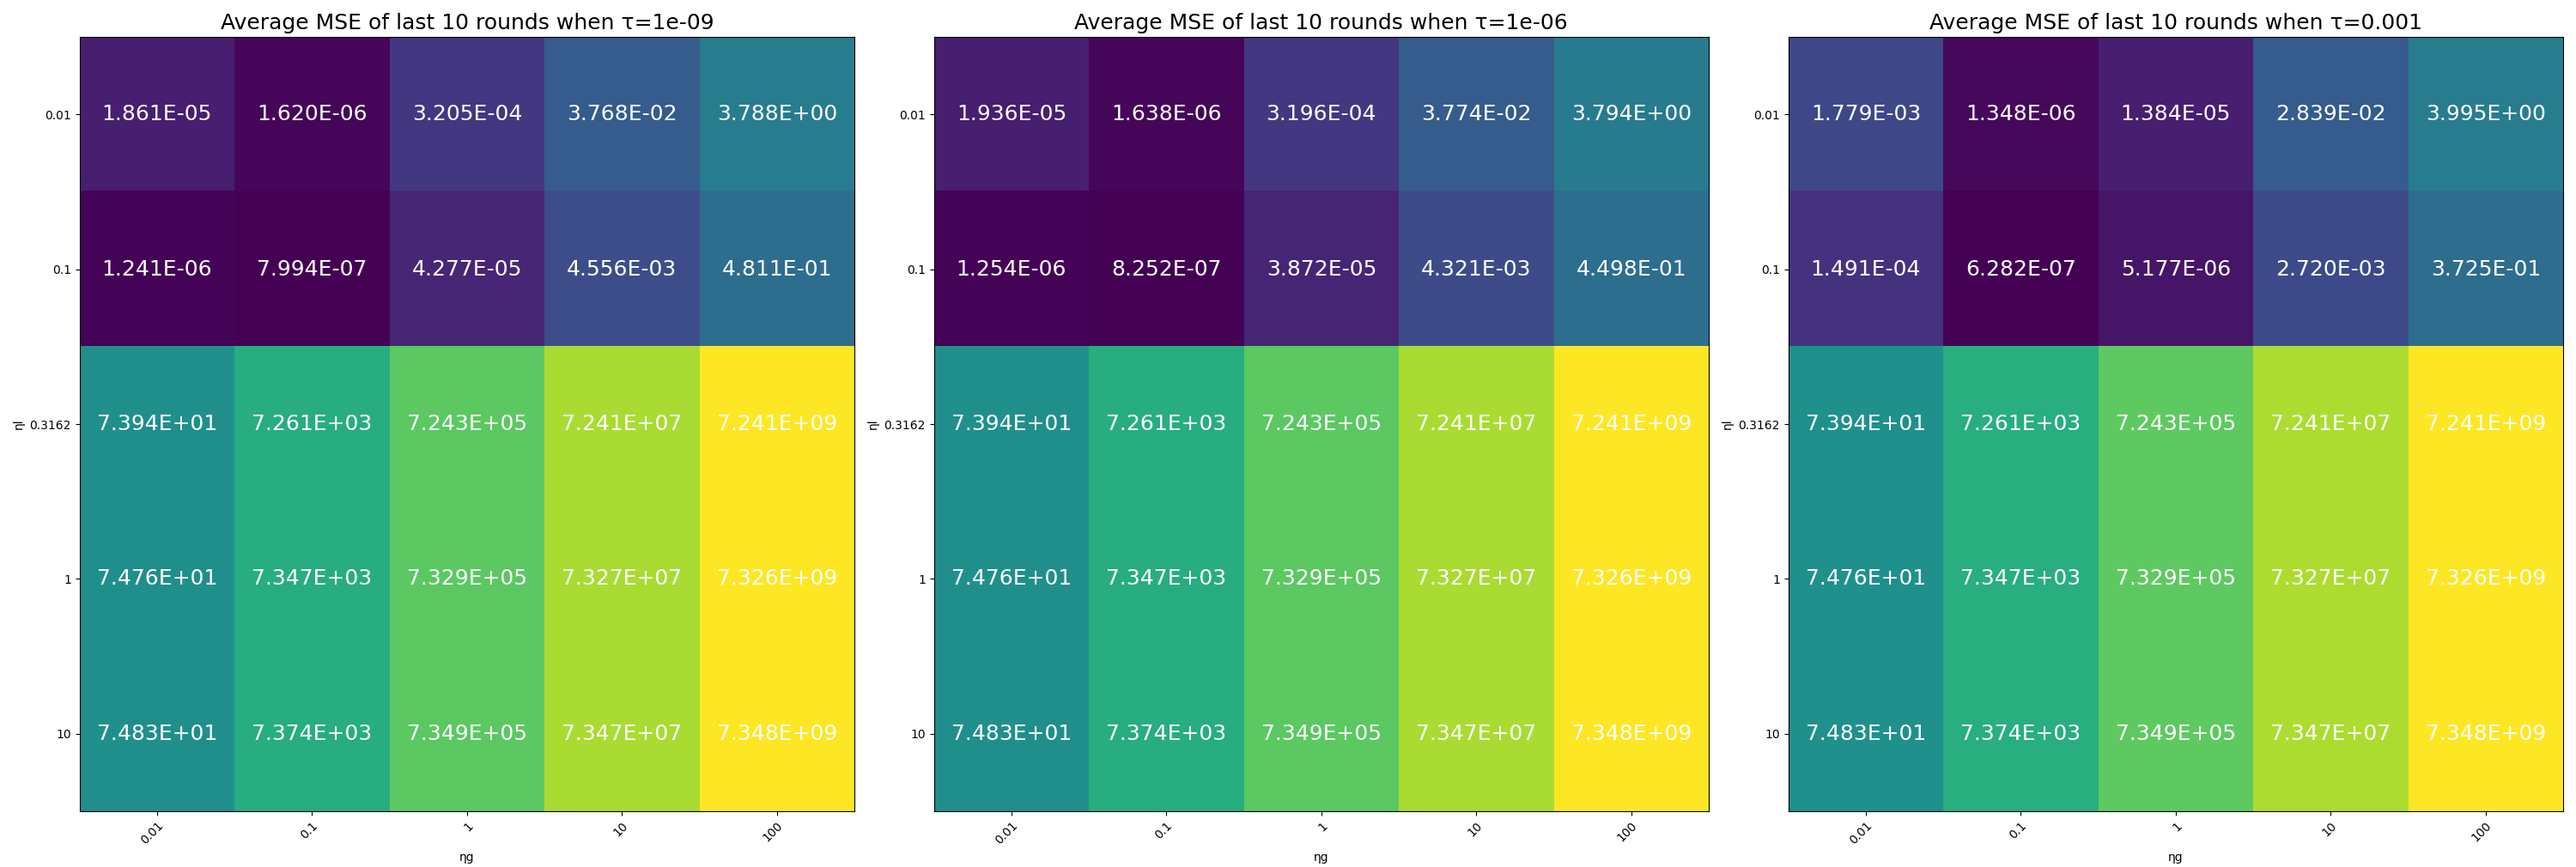
\includegraphics[width=\linewidth]{figs/fedAdamSyntheticHyperpameterTuning.png}}
    \caption{Hyper-parameter sweep of FedAdam for the synthetic data set}
    \label{fig:fedAdamSweep}
\end{figure}

Hydra is used to allow easy management of the configuration of the runs of the baseline, and to manage the hyper-parameters -- this makes it very easy to be able to change any of the values which you may want to, for example the number size of mini-batches, number of local epochs, concentration of Dirichlet distribution etc., are all controlled by YAML config files the given versions will produce the same results as in the original FedExP paper (with the optimal hyper-parameters selected for each strategy).  The use of these configuration files makes it very easy to add in new strategies to the comparison on any data set and perform hyper-parameter tuning; FedAdam has been addded as an additional algorithm compared the original paper for use on the synthetic data set, to add it to the comparison a single new YAML file had to be created specifying where to find the strategy (the FedAdam strategy is already built into Flower so this is referencing that implementation), and the hyper-parameters associated with that strategy (but none of the general hyper-parameters which affect all strategies).  To perform a hyper-parameter sweep Hydra can be used in multi-run mode, where you specify several values for each hyper-parameter and the baseline is run across all combinations the results of the hyper-parameter sweep for FedAdam on the synthetic data set can be seen in figure \ref{fig:fedAdamSweep} (the values for $\beta_1$ and $\beta_2$ are kept at 0.9 and 0.99 respectively, as was done in \cite{AdaptiveFederatedOptimisation}.

Also in this section I think I should show how it is easy to add FedAdam to comparison in synthetic dataset case and to perform the hyperparameter sweep to get good values for the hyper-parameters.


Also potentially need to change the CIFAR-100 to work in the same way as CIFAR-10 for generating the different distributions because that I think is how the paper does it, although this is likely not quite a realistic as the current method.


\section{Analysis}

In this likely talk about the interesting observed behaviours and how it is is different to other algorithms which is quite telling, such as the fact it is has a much more perturbed loss curve compared to FedAvg and also showing how changing several of the hyperparameters of it affects the overall result.

\section{Conclusion}

\bibliography{refs}

\end{document}
